%%=============================================================================
%% Selectie
%%=============================================================================

\chapter{\IfLanguageName{dutch}{Proof-of-concept}{Proof-of-concept}}%
\label{ch:proof-of-concept}

In dit hoofdstuk wordt de proof-of-concept besproken 
waarbij een beoordeling wordt gevormd van de omgevingen op basis van de performantie metingen.
Allereerst wordt de opzet van de proof-of-concepts voor beide omgevingen besproken.
Hierna worden de performantie metingen uitgevoerd voor beide omgevingen waarna de resultaten worden besproken.
Als laatste worden alle resultaten samengevat op zo het te bekijken of Bun een geschikte plaatsvervanger van Node.js kan zijn.

\subsection{Opzet proof-of-concept}
Voor de performantie te meten wordt er per omgeving 2 proof-of-concepts gemaakt. 
Deze metingen zullen worden uitgevoerd op een Mac mini met volgende specificaties:
\begin{itemize}
  \item De Apple M2 chip.
  \item 8GB aan unified memory.
  \item Het macOS Sonoma besturingssysteem
  \item 256GB aan SSD opslag.
  \item Versie 21 van Node.js.
  \item Versie 1.1.3 van Bun.
\end{itemize}
De eerste proof-of-concept zal bestaan uit een script dat het Quick Sort algoritme bevat. 
Deze zal dienen om de computationele verwerking van elke omgeving te beoordelen. Hierbij wordt rekening gehouden met volgende metingen:
\begin{itemize}
    \item De gemiddelde uitvoeringstijd.
    \item Het gemiddelde CPU-gebruik.
    \item Het maximale geheugengebruik.
\end{itemize}
Het Quick Sort algoritme zal een meegegeven array sorteren door een spil element te kiezen binnen de array, 
en hierna de array in 2 arrays opsplitsen. De eerste array zal elementen bevatten die kleiner zijn dan het spil element 
en de andere array zal elementen bevatten die groter zijn. 
De 2 arrays worden vervolgens telkens recursief gesorteerd met dezelfde methode om zo een gesorteerde array te bekomen.
In het codevoorbeeld ~\ref{code:quicksort} kan de code voor het Quick Sort algoritme gevonden worden.
Hierbij is er de mogelijkheid de grootte van de te sorteren array mee te geven via de command-line.

\begin{listing}[H]
    \centering
    \begin{minted}[bgcolor=bg,
        fontfamily=tt,
        linenos=true,
        numberblanklines=true,
        numbersep=5pt,
        gobble=0,
        framesep=2mm,
        tabsize=4,
        obeytabs=false,
        breaklines=true,
        mathescape=false
        samepage=false,
        showspaces=false,
        showtabs =false,
        texcl=false]{js}
const quickSort = (array) => {
  if (array.length <= 1) {
    return array;
  }

  let pivot = array[0];
  let smallArray = [];
  let bigArray = [];

  for (let index = 1; index < array.length; index++) {
    if (array[index] < pivot) {
      smallArray.push(array[index]);
    } else {
      bigArray.push(array[index]);
    }
  }

  return [...quickSort(smallArray), pivot, ...quickSort(bigArray)];
};

const args = process.argv.slice(1); // get length of array
let myArray = Array.from({ length: args[1] }, () =>
  Math.floor(Math.random() * 9)
);
quickSort(myArray);
        \end{minted}
        \caption{\label{code:quicksort}Code voorbeeld quicksort}
\end{listing}

Naast de computationele verwerking te meten, wordt ook performantie bij I/O-taken gemeten.
Dit wordt gedaan door een proof-of-concept op te stellen die een applicatie back-end voorstelt in de respectievelijke omgeving.
Hierbij kan een gebruiker een recensie creëren over een bepaald onderwerp. 
Binnen de proof-of-concepts zal hierbij getest worden met zowel een Postgres databank als een MySQL databank.
Hierbij wordt rekening gehouden met volgende metingen:
\begin{itemize}
    \item De gemiddelde uitvoeringstijd.
    \item Het gemiddelde CPU-gebruik.
    \item Het maximale geheugengebruik.
    \item De responstijd.
    \item Het aantal gelijktijdige connecties.
    \item Het aantal verzoeken.
    \item De gemiddelde installatietijd.
\end{itemize}
Bij de proof-of-concepts worden enkel de ingebouwde HTTP servers gebruikt om zo beïnvloeding van externe bibliotheken te vermijden.
Voor de binnengekomen data naar een database te schrijven wordt een Object Relational Mapper (ORM) gebruikt. 
Hierbij wordt persistentie bereikt door de objecten binnen de applicatie te koppelen met tabellen in de database \autocite{Lorenz2017}.
De ORM zal deze koppeling afhandelen en zo een abstractie creëren die de technische details van de mappingimplementatie verbergt \autocite{Lorenz2017}.
Binnen de applicatie zal voor beide omgevingen gebruikt gemaakt worden van het Sequelize ORM. Deze ondersteunt zowel Postgres als MySQL.
Hierbij worden eerst 3 modellen gemaakt die de volgende tabellen voorstellen in de databank:
\begin{itemize}
  \item Het User model dat een gebruiker voorstelt.
  \item Het Subject model dat een onderwerp voorstelt.
  \item Het Review model dat de recensie van een bepaalde gebruiker over een bepaald onderwerp voorstelt.
\end{itemize}
De code voor het model van de gebruiker is te vinden in ~\ref{code:User}. Deze bevat 3 kolommen namelijk: de primaire sleutel (id), voornaam en familienaam.
Doormiddel van de sync methode wordt dit model gesynchroniseerd met de database. 
Het model van het onderwerp is gelijkaardig aan de gebruiker zoals te zien is in ~\ref{code:Subject}. Het recensie model heeft bijkomend 
ook nog de 1-op-1 relatie met respectievelijk de gebruiker en het onderwerp.
Om deze relatie tot stand te brengen wordt de belongsTo methode gebruikt in ~\ref{code:Review}. 
Deze zal in de tabel een vreemde sleutel toevoegen naar respectievelijk de gebruiker tabel en het onderwerp tabel. 
\begin{listing}[H]
  \centering
  \begin{minted}[bgcolor=bg,
      fontfamily=tt,
      linenos=true,
      numberblanklines=true,
      numbersep=5pt,
      gobble=0,
      framesep=2mm,
      tabsize=4,
      obeytabs=false,
      breaklines=true,
      mathescape=false
      samepage=false,
      showspaces=false,
      showtabs =false,
      texcl=false]{js}
const { Model, DataTypes } = require("sequelize");

class User extends Model {}

async function UserInit(sequelize) {
  User.init(
    {
      id: {
        type: DataTypes.INTEGER,
        autoIncrement: true,
        primaryKey: true,
      },
      firstName: {
        type: DataTypes.STRING,
        allowNull: false,
      },
      lastName: {
        type: DataTypes.STRING,
      },
    },
    { sequelize, modelName: "User" }
  );
  await User.sync();
}

module.exports = {
  User,
  UserInit,
};
\end{minted}
\caption{\label{code:User}Code van het gebruiker model}
\end{listing}

\begin{listing}[H]
  \centering
  \begin{minted}[bgcolor=bg,
      fontfamily=tt,
      linenos=true,
      numberblanklines=true,
      numbersep=5pt,
      gobble=0,
      framesep=2mm,
      tabsize=4,
      obeytabs=false,
      breaklines=true,
      mathescape=false
      samepage=false,
      showspaces=false,
      showtabs =false,
      texcl=false]{js}
const { Model, DataTypes } = require("sequelize");

class Subject extends Model {}

async function SubjectInit(sequelize) {
  Subject.init(
    {
      id: {
        type: DataTypes.INTEGER,
        autoIncrement: true,
        primaryKey: true,
      },
      name: {
        type: DataTypes.STRING,
        allowNull: false,
      },
    },
    { sequelize, modelName: "Subject" }
  );
  await Subject.sync();
}

module.exports = {
  Subject,
  SubjectInit,
};
\end{minted}
\caption{\label{code:Subject}Code van het onderwerp model}
\end{listing}

\begin{listing}[H]
  \centering
  \begin{minted}[bgcolor=bg,
      fontfamily=tt,
      linenos=true,
      numberblanklines=true,
      numbersep=5pt,
      gobble=0,
      framesep=2mm,
      tabsize=4,
      obeytabs=false,
      breaklines=true,
      mathescape=false
      samepage=false,
      showspaces=false,
      showtabs =false,
      texcl=false]{js}
const { Model, DataTypes } = require("sequelize");
const { User } = require("./user.js");
const { Subject } = require("./subject.js");
class Review extends Model {}

module.exports = async (sequelize) => {
  Review.init(
    {
      id: {
        type: DataTypes.INTEGER,
        autoIncrement: true,
        primaryKey: true,
      },
      message: {
        type: DataTypes.STRING,
        allowNull: false,
      },
    },
    { sequelize, modelName: "Review" }
  );
  Review.belongsTo(User, { onDelete: "CASCADE" });
  Review.belongsTo(Subject, { onDelete: "CASCADE" });
  await Review.sync();
};
\end{minted}
\caption{\label{code:Review}Code van het recensie model}
\end{listing}

In de code ~\ref{code:Instantie} wordt een connectie aangemaakt met de databank met behulp van Sequelize. 
De benodigde configuratie wordt met behulp van de config en env-cmd packages opgehaald. Zo is de 
gebruikersnaam, databasenaam en de technologie van de database te vinden in de configuratie bestanden.
Voor zowel te kunnen werken met MySQL als Postgres wordt gebruikgemaakt van de packages: mysql2 en pg.
Het wachtwoord zal dankzij env-cmd opgehaald worden uit het environment om zo de veiligheid te waarborgen.
Deze configuratie wordt dan gebruikt om de connectie aan te maken en de tabellen te initializeren.
Nadien worden ook de gebruiker en onderwerp tabel opgevuld met voorbeeld data zoals te zien is in ~\ref{code:Seed}.

\begin{listing}[H]
  \centering
  \begin{minted}[bgcolor=bg,
      fontfamily=tt,
      linenos=true,
      numberblanklines=true,
      numbersep=5pt,
      gobble=0,
      framesep=2mm,
      tabsize=4,
      obeytabs=false,
      breaklines=true,
      mathescape=false
      samepage=false,
      showspaces=false,
      showtabs =false,
      texcl=false]{js}
const { Sequelize } = require("sequelize");
const configuration = require("config");
const doReviewMigration = require("./review");
const seed = require("./seeder");
const { UserInit } = require("./user");
const { SubjectInit } = require("./subject");
//config
const username = configuration.get("development.username");
const database = configuration.get("development.database");
const dialect = configuration.get("development.dialect");
const password = configuration.get("password");

let sequelize;
async function initializeSequelize() {
  sequelize = new Sequelize(database, username, password, {
    host: "localhost",
    dialect: dialect,
  });
  try {
    await sequelize.authenticate();
    console.log("Connection has been established successfully.");
  } catch (error) {
    console.error("Unable to connect to the database:", error);
  }
  await UserInit(sequelize);
  await SubjectInit(sequelize);
  await doReviewMigration(sequelize);
  await seed(sequelize);
  return sequelize;
}

function getSequelize() {
  if (!sequelize) {
    throw new Error("initialize sequelize");
  }
  return sequelize;
}

module.exports = {
  initializeSequelize,
  getSequelize,
};
\end{minted}
\caption{\label{code:Instantie}Code bij aanmaken instantie sequelize}
\end{listing}

\begin{listing}[H]
  \centering
  \begin{minted}[bgcolor=bg,
      fontfamily=tt,
      linenos=true,
      numberblanklines=true,
      numbersep=5pt,
      gobble=0,
      framesep=2mm,
      tabsize=4,
      obeytabs=false,
      breaklines=true,
      mathescape=false
      samepage=false,
      showspaces=false,
      showtabs =false,
      texcl=false]{js}
async function seed(sequelize) {
  // Go to original state
  await sequelize.models.User.destroy({ truncate: { cascade: true } });
  await sequelize.models.Subject.destroy({ truncate: { cascade: true } });
  await sequelize.models.User.create({
    id: 1,
    firstName: "Quinten",
    lastName: "De Wolf",
  });
  await sequelize.models.Subject.create({
    id: 1,
    name: "Cars",
  });
  await sequelize.models.Subject.create({
    id: 2,
    name: "Planes",
  });
  await sequelize.models.Subject.create({
    id: 3,
    name: "Racing",
  });
}
module.exports = seed;
\end{minted}
\caption{\label{code:Seed}Code bij het opvullen van de tabellen}
\end{listing}

Als laatste wordt de server aangemaakt om een POST methode op het review endpoint aan te nemen.
In ~\ref{code:NodeServer} wordt de code om dit te bereiken in Node.js getoond. Hierbij komt data in de vorm van JSON binnen.
Deze bevat de recensie in combinatie met het id van het onderwerp en de gebruiker.
Deze zal dan gebruikt worden om een nieuwe rij aan te maken in de recensie tabel.

\begin{listing}[H]
  \centering
  \begin{minted}[bgcolor=bg,
      fontfamily=tt,
      linenos=true,
      numberblanklines=true,
      numbersep=5pt,
      gobble=0,
      framesep=2mm,
      tabsize=4,
      obeytabs=false,
      breaklines=true,
      mathescape=false
      samepage=false,
      showspaces=false,
      showtabs =false,
      texcl=false]{js}
const http = require("node:http");
const { initializeSequelize } = require("./sequelize.js");
async function main() {
  const sequelizeInstance = await initializeSequelize();
  http
    .createServer(async (req, res) => {
      if (req.method === "POST" && req.url === "/review") {
        let body = "";
        req.on("data", (data) => {
          body += data.toString(); // Convert buffer to string
        });
        req.on("end", async () => {
          try {
            const data = JSON.parse(body);
            // Validate data using @hapi/joi or any other validation library
            // For simplicity, let's assume the data is valid
            await sequelizeInstance.models.Review.create(data);
            res.writeHead(201, { "Content-Type": "application/json" });
            res.end();
          } catch (error) {
            console.error("Error:", error);
            res.writeHead(400, { "Content-Type": "application/json" });
            res.end(JSON.stringify({ message: "Invalid data" }));
          }
        });
      }
    })
    .listen(3000);
}
main();
\end{minted}
\caption{\label{code:NodeServer}Code om de requests te ontvangen}
\end{listing}
\subsection{Uitvoering metingen}
Voor de metingen wordt gebruikgemaakt van 2 hulpprogramma's: Hyperfine en Bombardier.
In \ref{code:HyperfineScript} wordt Hyperfine gebruikt om de gemiddelde uitvoeringstijd over verschillende iteraties van het script te berekenen.
Ook zal Hyperfine gebruikt worden om de gemiddelde installatietijd van de respectievelijke package managers te vergelijken zoals 
te zien is in \ref{code:HyperfineInstall}. Specifiek wordt de installatietijd bekeken wanneer het cache geheugen data bevat.
Bij de metingen wordt telkens versie 1.18 van Hyperfine gebruikt.
\begin{listing}[H]
  \centering
  \begin{minted}[bgcolor=bg,
      fontfamily=tt,
      linenos=true,
      numberblanklines=true,
      numbersep=5pt,  
      gobble=0,
      framesep=2mm,
      tabsize=4,
      obeytabs=false,
      breaklines=true,
      mathescape=false
      samepage=false,
      showspaces=false,
      showtabs =false,
      texcl=false]{shell-session}
      > hyperfine 'node index.js 1000' 'bun index.js 1000'
      \end{minted}
      \caption{\label{code:HyperfineScript}Gebruik Hyperfine commando bij het script}
\end{listing}

\begin{listing}[H]
  \centering
  \begin{minted}[bgcolor=bg,
      fontfamily=tt,
      linenos=true,
      numberblanklines=true,
      numbersep=5pt,  
      gobble=0,
      framesep=2mm,
      tabsize=4,
      obeytabs=false,
      breaklines=true,
      mathescape=false
      samepage=false,
      showspaces=false,
      showtabs =false,
      texcl=false]{shell-session}
      > hyperfine --prepare 'rm -rf node_modules' --warmup 1 --runs 10 'npm install' 'bun install'
      \end{minted}
      \caption{\label{code:HyperfineInstall}Gebruik Hyperfine commando bij het script}
\end{listing}
Daarnaast wordt voor de HTTP server gebruik gemaakt van Bombardier. 
Hierbij kan ingesteld worden hoeveel gelijktijdige connecties er zijn en hoeveel verzoeken per test worden verstuurd.
In de metingen zal getest worden door 500000 verzoeken te sturen met 10, 100 en 1000 gelijktijdige connecties.
De commando's hiervoor zijn terug te vinden in \ref{code:Bombardier10}, \ref{code:Bombardier100} en \ref{code:Bombardier1000}.
Bij de metingen wordt hiervoor gebruikgemaakt van versie 1.2.6 van Bombardier.
\begin{listing}[H]
  \centering
  \begin{minted}[bgcolor=bg,
      fontfamily=tt,
      linenos=true,
      numberblanklines=true,
      numbersep=5pt,  
      gobble=0,
      framesep=2mm,
      tabsize=4,
      obeytabs=false,
      breaklines=true,
      mathescape=false
      samepage=false,
      showspaces=false,
      showtabs =false,
      texcl=false]{shell-session}
      > bombardier -c 10 -n 500000 -m POST -b "{'message': 'test','UserId': 1,'SubjectId': 1}" -l http://localhost:3000/review
      \end{minted}
      \caption{\label{code:Bombardier10}Gebruik Bombardier commando met 500000 verzoeken en 10 gelijktijdige connecties}
\end{listing}
\begin{listing}[H]
  \centering
  \begin{minted}[bgcolor=bg,
      fontfamily=tt,
      linenos=true,
      numberblanklines=true,
      numbersep=5pt,  
      gobble=0,
      framesep=2mm,
      tabsize=4,
      obeytabs=false,
      breaklines=true,
      mathescape=false
      samepage=false,
      showspaces=false,
      showtabs =false,
      texcl=false]{shell-session}
      > bombardier -c 100 -n 500000 -m POST -b "{'message': 'test','UserId': 1,'SubjectId': 1}" -l http://localhost:3000/review
      \end{minted}
      \caption{\label{code:Bombardier100}Gebruik Bombardier commando met 500000 verzoeken en 100 gelijktijdige connecties}
\end{listing}
\begin{listing}[H]
  \centering
  \begin{minted}[bgcolor=bg,
      fontfamily=tt,
      linenos=true,
      numberblanklines=true,
      numbersep=5pt,  
      gobble=0,
      framesep=2mm,
      tabsize=4,
      obeytabs=false,
      breaklines=true,
      mathescape=false
      samepage=false,
      showspaces=false,
      showtabs =false,
      texcl=false]{shell-session}
      > bombardier -c 1000 -n 500000 -m POST -b "{'message': 'test','UserId': 1,'SubjectId': 1}" -l http://localhost:3000/review
      \end{minted}
      \caption{\label{code:Bombardier1000}Gebruik Bombardier commando met 500000 verzoeken en 1000 gelijktijdige connecties}
\end{listing}
Als laatste wordt het ingebouwde commando time gebruikt om het cpu-gebruik en geheugengebruik te meten bij de proof-of-concepts.
\subsection{Resultaten proof-of-concept}
In deze sectie zullen de resultaten van de performantie testen besproken worden.
Hierbij worden eerst de resultaten voor de uitvoeringstijd, cpu-gebruik en geheugengebruik bij het Quick Sort algoritme bekeken.
Daarna worden de resultaten van de server besproken op vlak van uitvoeringstijd, cpu-gebruik, geheugengebruik, responstijd en de installatietijd.

\subsubsection{Resultaten Quick Sort algoritme}
De resultaten voor de gemiddelde uitvoeringstijd bij het Quick Sort algoritme werden bekomen doormiddel van Hyperfine.
Hierbij werd gekeken naar de uitvoeringstijd voor het sorteren van een array bestaande uit 1000 elementen met volgend commando \ref{code:HyperfineScript}.
In figuur \ref{fig:uitvoeringstijdscript} wordt de gemiddelde uitvoeringstijd per omgeving visueel voorgesteld. 
Daarbij is op te merken dat de gemiddelde uitvoeringstijd van Bun gemiddeld 2.21 keer sneller is dan bij Node.js.
\begin{figure}[H]
  \centering
  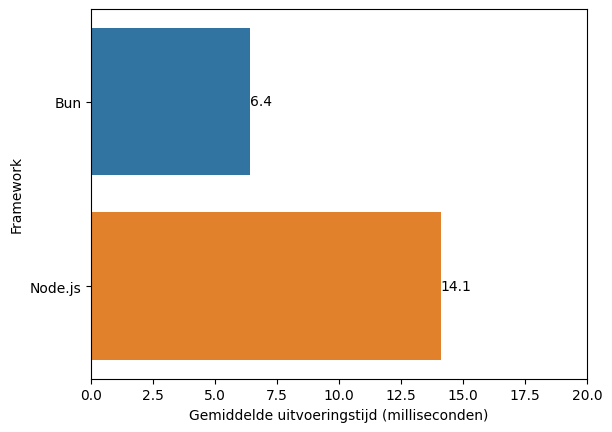
\includegraphics{graphics/scriptuitvoeringstijd.png}
  \caption{\label{fig:uitvoeringstijdscript}Gemiddelde uitvoeringstijd bij het Quick Sort algoritme voor Bun en Node.js}
\end{figure}